\documentclass[pra,11pt]{revtex4-1}
\usepackage[english]{babel}
\usepackage[utf8]{inputenc}
\usepackage{graphicx}
\usepackage{comment}
\usepackage{hyperref}
\usepackage{xypic}
\usepackage{subfig}
\usepackage{color}
\usepackage{array} % vertical centering in tabular
\usepackage{amsmath,amssymb,amsfonts} 

\begin{document}

\section{Symmetric dissociation of the water molecule}

\begin{itemize}
	\item Searching for more difficult test case than H$_4$
	\item Limited by FCI size of 4 orbitals $\rightarrow$ symmetric dissociation of H$_2$O
	\item Breaking of two bonds, correct description requires 4 orbitals in the active space
	\item Testing of the smallest non-trivial ($M = 1$ corresponds to the HF state) MPS: $M = 2$ 
	\item The advantage is that $M = 2$ MPSs can be easily prepared with just one ancilla qubit
\end{itemize}

\begin{figure}[!h]
  \subfloat[][]{
  \hskip -1cm
    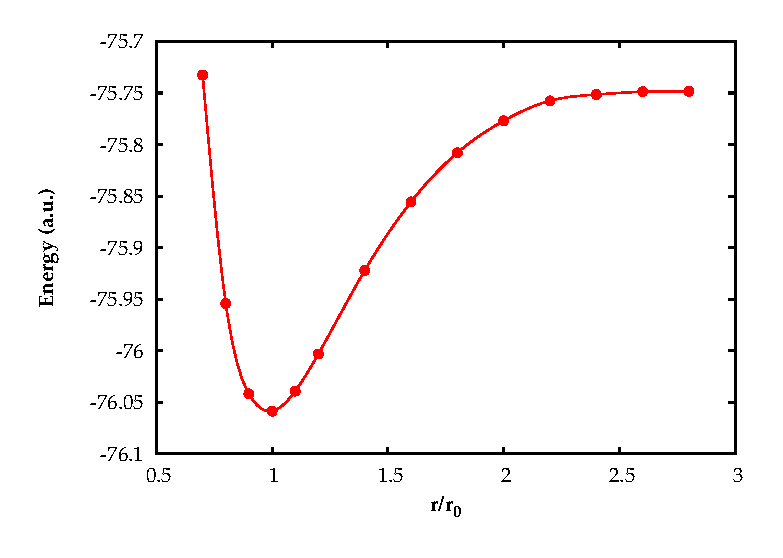
\includegraphics[width=9cm]{energy.eps}
    \label{en_disociace}
  }
  \subfloat[][]{
    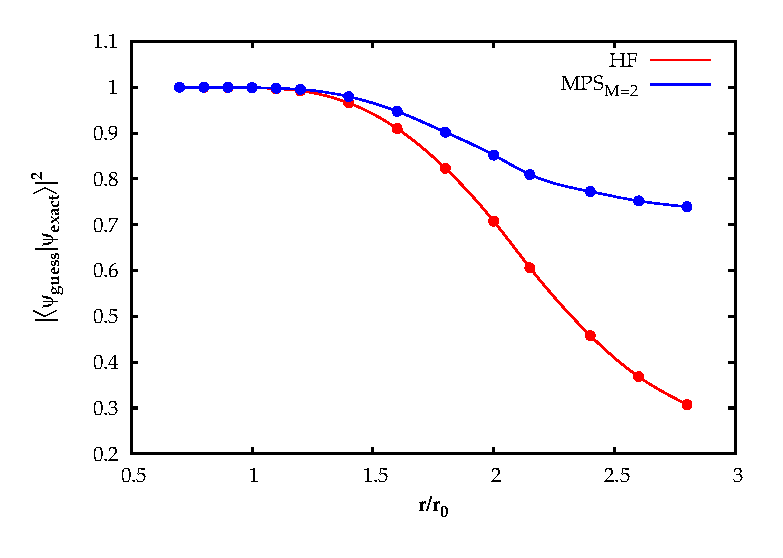
\includegraphics[width=9cm]{overlap.eps}
    \label{en_bending}
  }
  \caption{Water dissociation in cc-pVTZ basis.}
\end{figure}

In what follows, I denote standard variational eigenvalue solver (with $i$, $a$ indices) as VQE and the generalized one (with $p$, $q$ indices, i.e. all terms of the Hamiltonian) as generalized VQE.

\begin{enumerate}
	\item Test VQE (e.g. with MP2 guess for amplitudes) with HF initial state, plot the energy errors (with respect to FCI) for the whole dissociation curve - problematic should probably be the region with large $r$.
	\item Test VQE with the exact guess amplitudes extracted from the FCI wave function and HF initial state - should coverge faster.
	\item Test VQE with the exact amplitudes (for fast convergence) and MPS initial state to confirm, that the energy is exactly the same as with the HF initial guess (point 2).
	\item Test if MPS amplitudes can be helpfull with standard VQE.
	\item Test generalized VQE with the exact amplitudes (for fast covergence, amplitudes corresponding to operators annihilating the HF reference will be set to $0$ in the guess) and HF initial state. Compare the energies with standard VQE (point 2).
	\item Test generalized VQE as in the previous point, but with MPS initial state to see if the convergence is faster and energy better.
	\item Test the same as in the previous point, but with MPS amplitudes.
\end{enumerate}

\end{document}

